\documentclass[12pt,a4paper]{article}
\usepackage[utf8]{inputenc}
\usepackage[T1]{fontenc}
\usepackage[ngerman]{babel}
\usepackage{amsmath}
\usepackage{amsfonts}
\usepackage{amssymb}
\usepackage{lmodern}
\usepackage{tikz-uml}

\newcommand*{\Title}{Projektseminar: Gestensteuerung einer 3D-Anwendung mittels Kinect}
\newcommand{\Authors}{Mario Janke,\\Peter Lindner,\\Patrik Stäblein}
\title{\Title}
\author{
	Mario Janke\\
	Peter Lindner\\
	Patrik Stäblein}
\date{}

\usepackage{fancyhdr}
\usepackage{vmargin}
\usepackage{setspace}
\onehalfspacing
\pagestyle{fancy}  %lustige fuß- und kopfzeilen
\parindent 0pt	
\parskip 0pt %
\emergencystretch 20pt
\setmarginsrb{3.0cm}{2.5cm}{2.5cm}{1.5cm}%  %ränder links oben rechts unten
             {1.0cm}{1.5cm}{1.0cm}{1.7cm}%  %kopf und fußzeile, höhe, abstand
\setlength{\leftmargin}{3.0cm}
\setlength{\textwidth}{15.5cm}
\setlength{\headwidth}{15.5cm}
\setlength{\topmargin}{2.0cm}
\lfoot{\footnotesize{\emph{\Title}}}
\cfoot{}
\rfoot{\footnotesize{\emph{\thepage}}}
\rhead{\emph{\leftmark}}
\chead{}
\lhead{}
\renewcommand{\footrulewidth}{0.5pt}
\renewcommand{\headrulewidth}{0.5pt}

\begin{document}
\maketitle
\tableofcontents
\clearpage
\section{Rahmenbedingungen}
	\subsection{Grundlagen und Motivation}
	Gegeben ist eine bereits vorhandene 3D-Anwendung, die vom Betreuer des Projektseminars, Herrn M.\,sc. Julian Meder, erstellt wurde. Das Programm wird zu Demonstrationszwecken z.\,B. am Tag der offenen Tür in den Räumlichkeiten des Fachgebiets genutzt. Innerhalb der Anwendung ist es möglich,
	\begin{itemize}
		\item Objekte einzuladen und anzeigen zu lassen sowie
		\item die Kamera (bzw. Kameras) zu manipulieren, d.\,h. zu bewegen, zu rotieren und zu zoomen.
	\end{itemize}
	In Erweiterung soll das Programm auch weiteren Aufgaben der Objektmanipulation dienlich sein, dies beinhaltet insbesondere das Laden mehrerer Objekte in eine Szene und die Manipulation dieser im Sinne von Translation, Rotation, Skalierung und Löschung.\par
	Den oben genannten Demonstrationszweck nimmt das Programm über die Ankopplung des Rechners an einen 3D-Kameraaufbau wahr. Das Programm rendert zwei Ausgabefenster aus zwei verschiedenen, im Sinne der Stereoskopie angeordneten Kamerasichten. Dies wird von den beiden Projektoren im Nebenraum des Päsentationsraums genutzt um ein linkes und ein rechtes Bild von hinten auf einen Schirm zu strahlen, der in die Trennwand der beiden Räume eingelassen ist. Mittels handelüblicher aus 3D-Kinos bekannten Shutterbrillen können Benutzer und Zuschauer sodann den 3D-Eindruck wahrnehmen.\par
	Die Steuerung des genannten Grundprogramms erfolgt durch den Vortragenden (im Weiteren zumeist Master genannt) über Tastatur und Maus bzw. einen Präsentationspointer. Die Unhandlichkeit sowie fehlende Immersion und Attraktivität dieser Steuerung ist eine Kernmotivation für unser Projekt. Darüber hinaus motivierend ist auch die bloße Auseinandersetzung mit der am Fachgebiet vorhandenen Technik sowie die Untersuchung der Möglichkeiten, diese zielführend einzusetzen.
	\subsection{Eigenschaften der Kinect} 
	Wir stellen in diesem Abschnitt nur die für uns interessanten Eigenschaften und Möglichkeiten der Kinect vor (hinsichtlich unserer Aufgabe und der Rahmenbedingungen). Die Kinect erkennt visuell den 3D-Raum vor sich. Dabei werden Personen als solche detektiert und konfidenzbasiert mit einem primitiven und grobgranularen Skelett ausgestattet. Dieses Tracking ist für bis zu sechs Personen zeitgleich möglich. Weiterhin wird für beide Hände einer getrackten Person ein \glqq Handzustand\grqq~erkannt, nämlich ob die Hand offen oder geschlossen ist, oder die sogenannte Lassogeste gebildet wird (etwa nur zwei Finger ausgestreckt). Kann einer Hand keiner dieser Zustände zugeordnet werden, ist ihr Status unbekannt. Diese Daten (Skelett und Status pro getrackter Person) können unter Verwendung der USB-Schnittstelle und des Kinect-SDKs abgegriffen werden. Sie werden dafür 30 mal in der Sekunde zur Verfügung gestellt.
	%
	%
\section{Vorüberlegungen}
	Für unser Vorgehen zentral sind die folgenden beiden Bereiche:
	\begin{enumerate}
		\item die technische Umsetzung, d.\,h.
		\begin{itemize}
		\item das korrekte Erkennen und Werten von Gesten einer ausgezeichneten getrackten Person
		\item das korrekte Berechnen notwendiger Bewegungsparameter
		\item die Einbindung in die bestehende Applikation
		\end{itemize}
		\item die Interaktion mit dem Benutzer, d.\,h.
		\begin{itemize}
		\item das Entwerfen intuitiver und eingängiger Gesten für die verschiedenen Zwecke
		\item das Auszeichnen einer getrackten Person als \glqq Master\grqq, der das Programm steuert
		\end{itemize}
	\end{enumerate}
	Wir stellen in diesem Abschnitt die zentralen unmittelbaren Beobachtungen vor, die sich aus der Aufgabenstellung und dem Versuchsaufbau ziehen lassen.\par\bigskip
	Ausgehend von der Aufgabenstellung kann man abstrahierend zwischen zwei primitiven Steuerungsmodi unterscheiden:
	\begin{itemize}
	\item einem Modus, in dem die Kamera verschoben und rotiert werden kann \&
	\item einem Modus, in welchem Objektmanipulationen möglich sind.
	\end{itemize}
	Der Benutzer sollte sich zu jedem Zeitpunkt nur in maximal einem dieser Modi aufhalten, d.\,h. gleichzeitige Kamera- und Objektmanipulation wird ausgeschlossen. Diese Vereinfachung treffen wir, da damit weniger komplexe Gesten benötigt werden und eine solche simultane Manipulation keine praktische Relevanz besitzt. Für Manipulationen, die man sowohl für die Kamera, als auch für Objekte haben will, bietet dies zudem eine geeignete Kapselung, da z.\,B. Rotationsparameter berechnet werden und dann nur entschieden werden muss, ob sie auf die Kamera oder ein Objekt angewendet werden, je nach Modus. Dies reduziert die Gesamtzahl nötiger Gesten.\par\medskip
	Die Kinect ermöglicht ein Tracking des gesamten Körpers für mehrere (genauer sechs) Personen. Wir beschränken uns aus naheliegenden Gründen jedoch auf einen Teil dieses Spektrums:
	\begin{itemize}
		\item Wir benötigen nur eine Person, die die Anwendung (möglichst ungestört) steuert. Eine genauere Auswertung der restlichen Personen, ihrer Skelette etc. ist unnötig.
		\item Die in unserem Anwendungsfall intuitiven Gesten werden ausschließlich mit den Händen (bzw. Armen) durchgeführt.
	\end{itemize}
	Primitive Erkennungsmöglichkeiten eines Masters kann man etwa aus der Entfernung der getrackten Personen zur Kamera und der Position der Personen im Raum gewinnen. Genauere Erklärungen folgen weiter unten.\par 
	Intuitive Gesten für Verschiebungen imitieren das Verschieben eines großen Gegenstands, etwa einer imaginären Box, sodass hier etwa ein Verschieben der flachen Hand in der Luft naheliegt. Für eine intuitive Drehgeste eignet sich die Vorstellung eines imaginären Lenkrads, genauer gesagt einer Lenkkugel, bei der die Rotation um eine Raumachse nach dem Lenkradprinzip erfolgt. Eine intuitive Geste zur Objektauswahl ist offenbar eine Greifgeste.
	%
	%
\section{Entwurfsentscheidungen}
	\subsection{Der Master}
	Der Master ist die Person (unter den getrackten Personen), der es obliegt, die Anwendung zu steuern, d.\,h. in unserem Anwendungsfall der Präsentation ist der Master der Präsentierende.\par
	Es muss gewährleistet werden, dass nur der Master das Programm steuert und dabei von weiteren Personen im Raum nicht (bzw. nicht ohne weiteres) gestört werden kann. Die Erkennung muss robust gegen Jittering der Kinectdaten sein.
	\subsection{Gesten und ihre Wirkung}
	Für die eingangs erwähnte Aufgabenstellung war es notwendig, bestimmte Programmfunktionalitäten mit Gesten zu verbinden. Einerseits hätte die Möglichkeit bestanden, mit dem Kinect-eigenen Visual Gesture Builder Gesten aufzunehmen und einzulernen. Diese Gesten werden dann als Datenbank ins Programm geladen und bei Vorführung erkannt. Dies erspart natürlich primitive aber umständliche Low-Level-Erkennungsmechanismen. Weiterhin sind hierdurch einige weiterführende Möglichkeiten gegeben wie etwa die Rückgabe, bis zu welchem Punkt eine Geste bereits ausgeführt wurde (in Bezug zur Gesamtgeste, d.\,h. beispielsweise wieviel Prozent einer Armbewegung vordefinierte Länge bereits ausgeführt wurde). Anderseits wiederum können durch die Kinect-Rohdaten auch eigene Erkennmechanismen implementiert werden. Dies bietet dem Programmierer die vollständige Kontrolle über seinen Gestenkatalog. Änderungen können kurzfristig und schnell vorgenommen werden und für einfache Projekte ist die Zusatzfunktionalität, die der Visual Gesture Builder gestattet nicht vonnöten, der eher für komplexere Gestenfolgen ausgelegt zu sein scheint. Demgegenüber ist für diese Direktimplementierung von Gesten aber die bereits erwähnte Low-Level-Erkennung zu implementieren, d.\,h. ein Extrahieren von Bewegungen und Bewegungsrichtungen aus den Skelett- und Gelenkdaten, die die Kinect bestimmt. Dennoch entschieden wir schließlich uns kraft dieser Gegenüberstellung (nebst einigen Versuchen mit dem Visual Gesture Builder, die uns nicht von seinem Mehrwert in unserer konkreten Anwendungssituation überzeugen konnten) für eine direkte Gestenerkennung.\par 
	Auch bei der Low-Level-Erkennung gibt es jedoch verschiedene Ansätze bzw. Ausprägungen. Es ist sogar das Implementieren nicht ganz primitiver Gestenfolgen möglich, indem eine Geste zeitlich und räumlich in verschiedene Segmente unterteilt wird. Dies sei an einem Beispiel erläutert: Es soll eine Winkgeste der rechten Hand erkannt werden. Die Geste wird in zwei Segmente geteilt. Ein Wechsel zwischen den Segmenten findet statt, wenn die horizontale Position der Hand und des Ellenbogens wechseln. Wird dieser Übergang dreimal in Folge erkannt, so wurde die Winkgeste präsentiert.\par
	Eine genauere Auseinandersetzung mit der Aufgabenstellung und unseren Vorstellungen von intuitiven Gesten für die zu realisierenden Funktionalitäten zeigte jedoch auf, dass auch eine Segmenteinteilung von Gesten für das Projekt nicht notwendig ist. Stattdessen sind die gegebenen Aufgaben in ihrer Struktur simpel genug, um die verschiedenen Wirkungen mit diskreten Gesten zu erzeugen, d.\,h. es genügt die Erkennung einer Geste durch bestimmte Zustände der Kinect-Rohdaten zu einem einzigen Zeitpunkt. Um die Wirkung jedoch zu erzielen, ist natürlich auch eine Betrachtung der Geste über mehrere Frames notwendig.\par\medskip
	Im Folgenden erklären wir unseren Gestenkatalog und gehen dabei darauf ein, was der Benutzer vorführen muss, damit die Geste erkannt wird und wie die Geste genutzt wird, um in der Anwendung die Kamera oder Objekte zu manipulieren:\par\bigskip
	\begin{description}
		\item[TRANSLATE\_GESTURE] (siehe Abb. \ref{fig:translateg})\par
		Der Benutzer hat beide Hände geöffnet, mit den Handflächen zur Kamera (wichtig ist nur, dass die Kinect beide Hände als offen erkennt, die genaue Haltung ist dabei egal). Ein paralleles Verschieben der beiden Hände in eine Richtung bewirkt ein zur Bewegungsgeschwindigkeit proportionales Verschieben der Kamera in diese Richtung.\par 
		Diese Geste war allen Projektteilnehmern unmittelbar einleuchtend und intuitiv und bedurfte keiner weiteren Diskussionen. 
		\begin{figure}[h!]
		\centering
		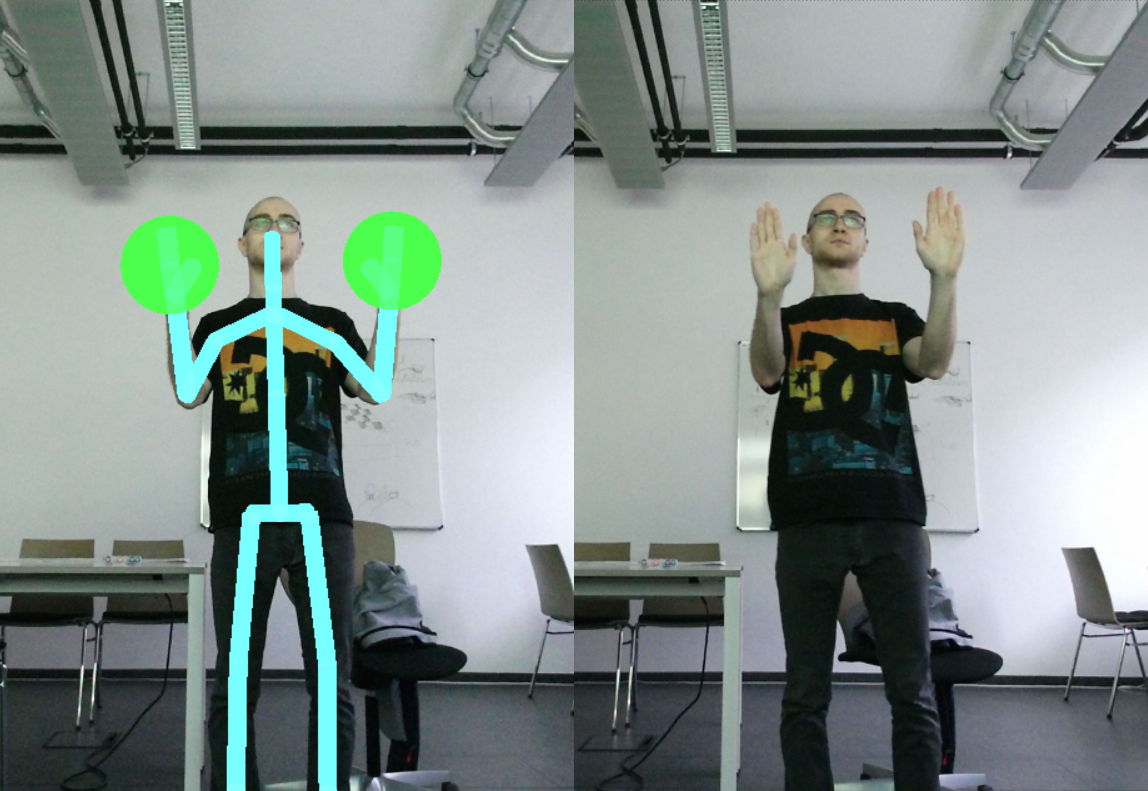
\includegraphics[width=.8\textwidth]{pictures/translate_.png}
		\caption{Die (Kamera-)Translations-Geste, mit und ohne eingezeichnetes Skelett und HandStates.}\label{fig:translateg}
		\end{figure}
		\par
		\item[ROTATE\_GESTURE] (siehe Abb. \ref{fig:rotateg})\par
		Der Benutzer hat beide Fäuste geballt. Dann bewirkt eine gleichzeitige Bewegung der Hände auf einer Kreisbahn eine Rotation der Kamera um die Senkrechte des zugehörigen Kreises. Dies ist genau die intuitive Art der Steuerung, mit der man etwa ein Aussichts- bzw. Münzfernrohr steuern würde.\par
		Wie die TRANSLATE-Geste war auch diese Geste von Anfang an im Team unumstritten.
		\begin{figure}[h!]
		\centering
		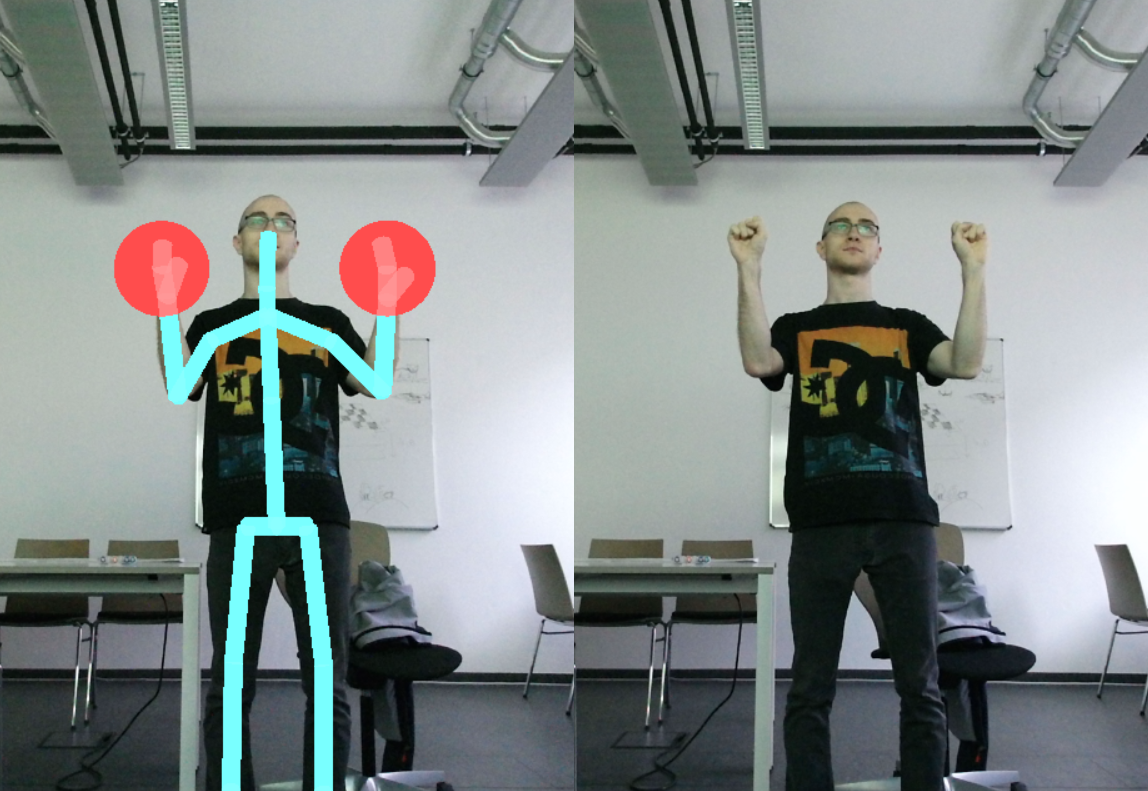
\includegraphics[width=.8\textwidth]{pictures/rotate_.png}
		\caption{Die (Kamera-)Rotations-Geste, mit und ohne eingezeichnetes Skelett und HandStates.}\label{fig:rotateg}
		\end{figure}		
		\par
		\item[GRAB\_GESTURE] (siehe Abb. \ref{fig:grabg})\par
		Zunächst war angedacht, dass die Objektmanipulation dieselben Gesten verwendet wie die Kameramanipulation und die Unterscheidung, was manipuliert wird durch einen globalen Zustand gefällt wird. Bei näherer Betrachtung dieses Ansatzes und ersten Tests dessen fiel auf, dass es so schwierig ist, zwischen Kamera- und Objektmanipulation zu wechseln. Weiterhin schien es während des Testens weniger intuitiv als zuvor angenommen, ein Objekt auf diese Art und Weise zu manipulieren. Es mussten also andere Ansätze gefunden werden.\par 
		In das Problem der Objektmanipulation eingeschlossen ist das Problem des Object-Pickings, d.\,h. die Auswahl des zu manipulierenden Objekts vom Bildschirm. Auch dies wäre mit der oben beschriebenen Methode, die die Gesten der Kameramanipulation verwendet, nur schwierig und umständlich realisierbar gewesen. Wir näherten uns dem Finden eines neuen Weges diesmal auf einem anderen Weg, nämlich nicht über die Manipulation, sondern über das Picking des Objekts. Schnell einigten wir uns auf das Greifen eines Objekts (eine Hand ist erhoben und geschlossen -- dies motiviert auch den Namen \glqq GRAB\grqq-Geste) als intuitivste Möglichkeit dafür. Von der Idee her sollte ein Hin- und Herbewegen dieser \glqq Kontroll-Hand\grqq{} auch das Objekt hin"= und herbewegen. Nachdem dies zufriedenstellend eingebaut war, widmeten wir uns der Objektrotation, was schnell eine fundamentale Schwäche dieser Geste offenbarte: Die Rotation des Objekts sollte der Rotation der geschlossenen Hand folgen, jedoch ist die Erkennung der Rotation einer geschlossenen Hand durch die Kinect viel zu schlecht, um an dieser Stelle sinnvoll Verwendung zu finden.\par 
		Die Ergebnisse wurden direkt sehr gut, als wir dazu übergingen, die GRAB"=Geste durch eine gehobene und offene (!) Hand zu definieren, da die Kinect so -- wie auch naheliegend -- viel besser erkennen kann, wie die Handfläche gekippt bzw. gedreht ist. Intern behielten wir jedoch den semantischen Namen \glqq GRAB\grqq"=Geste bei.
		\begin{figure}[h!]
		\centering
		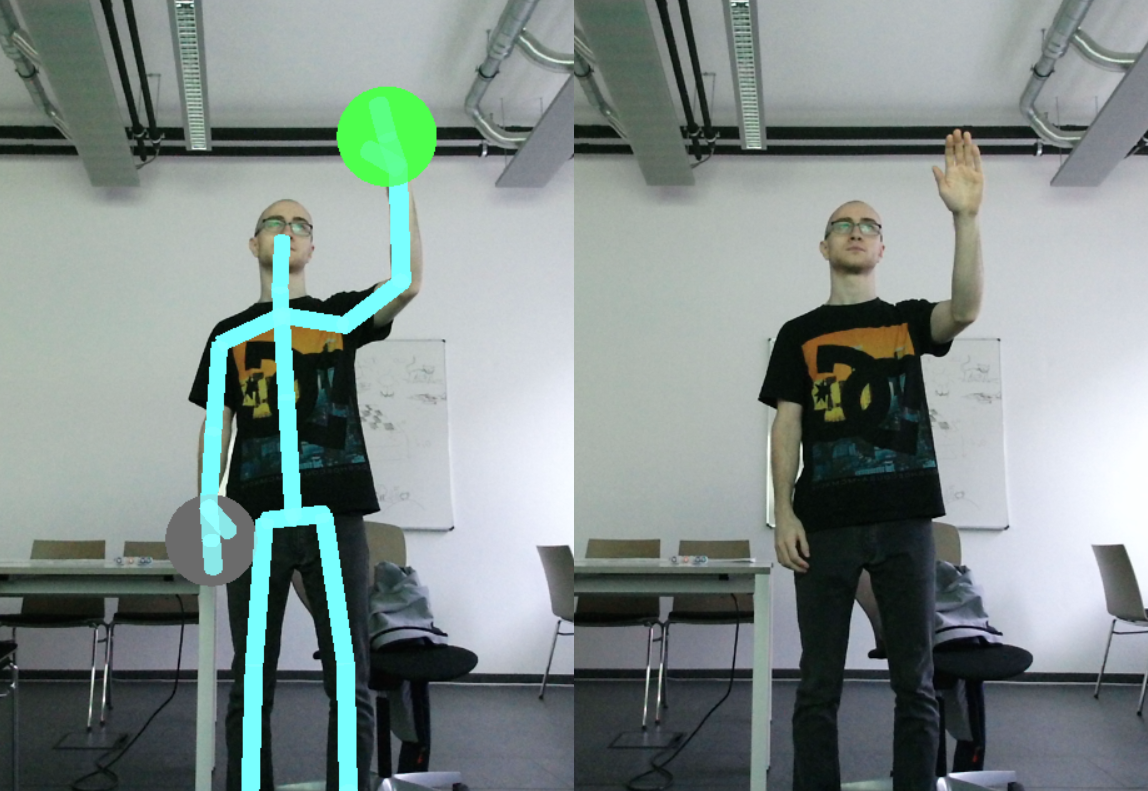
\includegraphics[width=.8\textwidth]{pictures/grab_.png}
		\caption{Die Objektmanipulations-Geste, mit und ohne eingezeichnetes Skelett und HandStates.}\label{fig:grabg}
		\end{figure}
		\par
		\item[FLY\_GESTURE] (siehe Abb. \ref{fig:flyg})\par
		Im Rahmen der Tests mit einem Beispielobjekt wurde schnell deutlich, dass es auch eine einfache Möglichkeit geben sollte, sich über weitere Strecken durch den Raum zu bewegen, ohne dabei ständig zwischen dem Vorführen einer Geste und einem \glqq Nachgreifen\grqq{} wechseln zu müssen. Als sinnvoll erschien hier, dass das Vorführen einer besonderen Geste bewirkt, dass die Kamera losfährt und erst anhält, wenn die Geste nicht mehr präsentiert wird.\par 
		Die FLY"=Geste entspricht dem Ausstrecken beider Arme vor den Körper, sodass sich die Hände mehr oder weniger am selben Punkt im 3D"=Raum befinden. Passiv findet bei dieser Geste im Programm eine Bewegung nach vorne statt. Durch Schwenken der Arme soll der Nutzer dabei die Richtung der Bewegung beeinflussen können, d.\,h. ein Zeigen der Arme nach oben bewirkt, dass die Bewegung immer weiter nach oben gezogen wird, während man mit einem Zeigen nach links oder rechts eine Kurve fliegen kann. Dabei bestimmt der Ausschlag der Arme beim Zeigen (verglichen mit der Ausgangsposition, in der beide Arme genau nach vorne gerichtet sind) die Stärke der Richtungsänderung. Um eine sogenannte Fassrole durchzuführen oder sich in Kurven legen zu können, kann der Nutzer nebenbei seine Schulterpartie in die entsprechende Richtung kippen. Insgesamt ist die Steuerung des Flugmodus in ihrem Funktionsumfang damit ähnlich zu üblichen Steuerungen von Flugzeugen in Actionspielen oder Simulationen.\par 
		Nicht zuletzt daher ist die assoziierte Geste für den Nutzer angenehm und intuitiv und ermöglicht eine im Gegensatz zur Bewegung über Drehen und Schieben einfache Möglichkeit, sich etwa durch ein System von Gängen in einer 3D"=Szene zu bewegen und generell Strecken zurückzulegen, statt Objekte zu betrachten. Ein, wenn auch in der Art der Gesamtanwendung begründetes Problem, ist jedoch, dass das Ausführen dieser Geste durch die nach vorne ausgestreckten Arme schnell anstrengend wird. Für Anwendungen, in denen -- nicht wie in unserem Fall -- der Hauptfokus tatsächlich auf dem Überwinden von längeren Strecken liegt, etwa in einem Rennspiel o.\,Ä., wäre es vermutlich notwendig, diesem Punkt erneut Beachtung zu schenken. Für unsere Aufgabenstellung ist die genannte Gestenvariante jedoch völlig ausreichend und besticht durch Intuition und Immersion.
		\begin{figure}[h!]
		\centering
		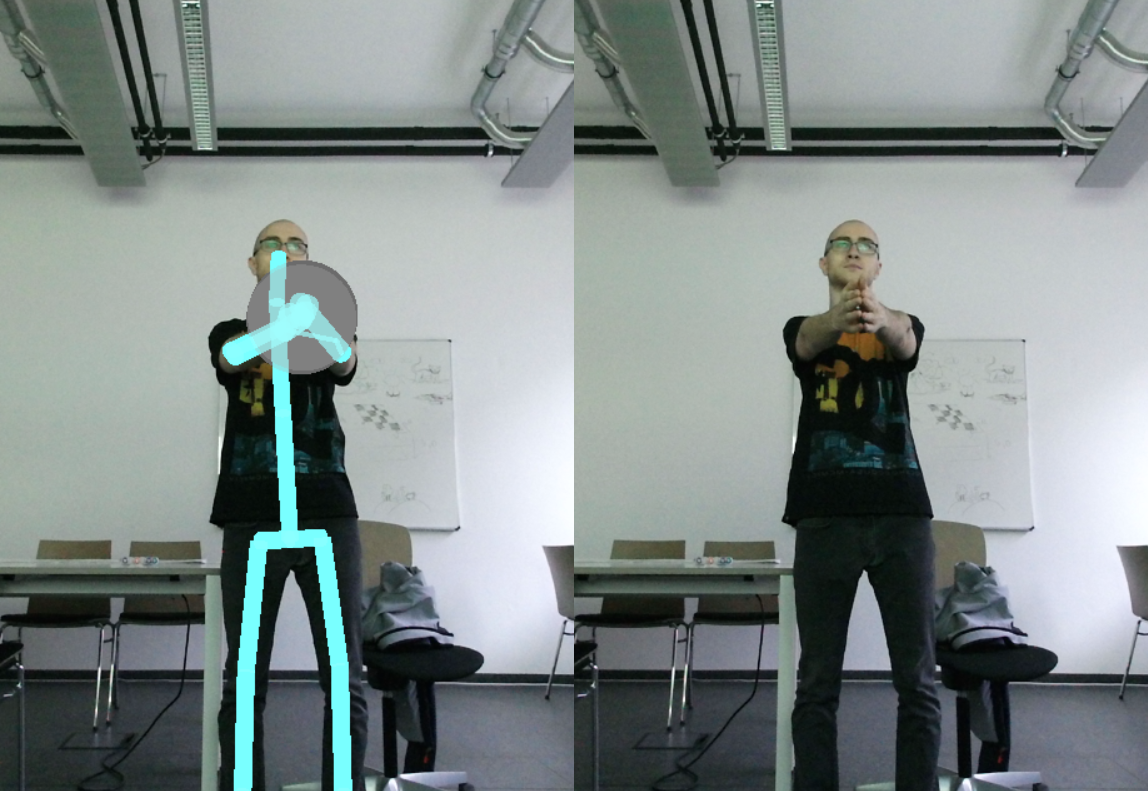
\includegraphics[width=.8\textwidth]{pictures/fly_.png}
		\caption{Die Flug-Geste, mit und ohne eingezeichnetes Skelett und HandStates.}\label{fig:flyg}
		\end{figure}\par		
		\item[UNKNOWN] Dies enthält alles, was als keine der anderen Gesten erkannt wird. Die Kamera und geladene Objekte sollen, solange diese Geste gezeigt wird, stillstehen.\par
		Neben der naheliegenden Motivation, dass der Nutzer die Szene gegebenenfalls auch bei Ruhe betrachten möchte, dient diese \glqq Geste\grqq{} (oder besser \glqq Nicht-Geste\grqq{}) darüber hinaus noch einem anderen Zweck. Sie kann in andere Gesten, wie beispielsweise Translationen, eingebaut werden, um diese aufzubrechen und \glqq nachgreifen\grqq{} zu können. Erst dies gestattet dem Nutzer, während der Bedienung an Ort und Stelle stehen bleiben zu können.
	\end{description}
	Tests mit der Kinect haben ergeben, dass es notwendig ist, bei derartig selbst implementierten Gesten auch eigene Robustheitsmechanismen einzubauen, die die Gestenerkennung gegen Schwankungen der Kinecterkennung (etwa des Status einer Hand) abhärten. Für genauere Informationen hierzu verweisen wir auf Abschnitt \ref{sec:robustheit}.
%
%
\section{Bemerkungen zum Quellcode}
		\subsection{Wichtige Datenstrukturen, Variablen und Funktionen}
		\subsection{Details zum Zusammenspiel}
		\subsection{Einbinden}
\end{document}